\section{Methods}

In this section, we first re-formulate the objective for the out-of-domain generalization by introducing an oracle model. Then, we derive a tractable variational bound of the objective by approximating the oracle model to the pre-trained model. The final form consists of the empirical risk and the mutual information (MI) regularization by querying the approximated oracle, named \fullname{} (\method{}). We empirically validate our approximation by MI between the oracle model and large pre-trained models. 

\subsection{Mutual information regularization with oracle}

% Introduction of Original DG
The main idea of the proposed method is to guide the learning process using oracle representations of training datasets.
In general, the problem of domain generalization (DG) is to find a model that minimizes an expected loss of \emph{any} domain by using training datasets from only partial domains, which are called source domains.
Many existing methods minimize an empirical loss averaged over source domains.
% To optimize a target model, many existing methods often minimize an empirical loss averaged over source domains.
More specifically, suppose that training samples $\{\mathcal{S}_{d}\}_{d=1}^{m}$ are given in $m$ domains and we consider a hypothesis set $\mathcal{H}$ for optimization.
Then, many existing DG frameworks can be formulated as follows:
% Then, \kj{[Check this sentence and formulation. Is it really general in DG?]} existing DG frameworks can be formulated as follows,
\begin{align}\label{eq:origin_dg}
  \bar{h}=\argmin_{h\in\mathcal{H}} \sum_{d=1}^{m} \mathcal E_{\mathcal{S}_{d}}(h),
\end{align}
where $d$ indicates an individual source domain and $\mathcal E_{\mathcal{S}_{d}}$ is an empirical loss over the source domain $d$.
Note that majority of existing DG methods can be interpreted as the variant of Equation \eqref{eq:origin_dg}.
For example, if we choose a simple cross-entropy loss for $\mathcal E_{\mathcal{S}_{d}}$, then Equation \eqref{eq:origin_dg} becomes ``ERM'' baseline used in \cite{gulrajani2020domainbed}\footnote{Note that the terminology ERM can be unfair because other methods also minimize ``empirical risk'' but with different loss designs. We use the terminology ``ERM'' to indicate the cross-entropy baseline as suggested by Gulrajani and Lopez-Paz \cite{gulrajani2020domainbed}.}. Otherwise, $\mathcal E_{\mathcal{S}_{d}}$ can be formulated as a regularized ERM, such as IRM \cite{arjovsky2019irm} or CORAL \cite{sun2016coral}.
However, the formulation \eqref{eq:origin_dg} still suffers from learning domain-invariant representations using only partial domains when the target distribution differs significantly from the training distribution. For example, CORAL, the state-of-the-art method, shows inconsistent out-of-domain accuracies across domains in DomainNet \cite{peng2019domainnet}. While CORAL achieves $\approx$50\% top-1 accuracy on four \emph{easy} domains (59.2\% for Clipart, 46.6\% for Painting, 59.8\% for Real, 50.1\% for Sketches), it only shows 13.4\% for QuickDraw and 19.7\% for Infographics where the domains show the significant distribution shift comparing to others.

% Problem Formulation
To alleviate this issue, we re-formulate the DG problem by employing \emph{oracle} representations of source domains. Here, we define an oracle model as a model that can be generalized to \emph{any} possible domain, not only for the source domains.
We define a model as a composition of a feature extractor $f$ and a classifier $g$ on the feature space where the whole classifier $h$ can be written as $h=f\circ g$.
Then, let $f^{*}$ be a feature extractor of the oracle model.
We first start from a strong assumption: 
we may assume that $f^*$ is accessible during the training phase. Then, we can obtain additional information from $f^{*}$ by querying the oracle representations of training samples in the source domains.
By using the oracle representations, we can guide the learning process of a target model by maximizing MI between oracle representations and target ones.
We formulate the proposed oracle-guided DG framework as follows:
% Hence, an oracle guided DG framework can be formulated as follows,
\begin{align}
\begin{split} % for single number
    \max_{h} \quad & I(Z_{f^\mathfrak{*}};Z_{f}) \\
    \textrm{s.t.} \quad & \mathcal{E}_{\mathcal S}(h) - \mathcal{E}_{\mathcal S}(\bar{h}) \leq \epsilon,
\end{split}
\label{eq:obj_constrained_mother}
\end{align}
where $Z_{f^{*}}$ is a random feature extracted by $f^{*}$ and $Z_{f}$ is a random feature extracted by a target model $f$. $I(Z_{f^{*}};Z_{f})$ is MI between $Z_{f^{*}}$ and $Z_{f}$, and $\mathcal{E}_{\mathcal S}(\cdot) = \sum_{d=1}^{m}\mathcal{E}_{\mathcal{S}_{d}}(\cdot)$.
% Note that, to define the mutual information between $Z_{f^{*}}$ and $Z_{f}$, we implicitly define a joint distribution of $(Z_{f^{*}},Z_{f})$ as the transformation of inputs such that $(Z_{f^{*}},Z_{f})=(f^{*}(X), f(X))$ for $X$ sampled from the distribution of source domains.
The inequality constraint ensures the performance of the target model on the source domains.
% We believe that the guidance of the oracle is beneficial to learning robust representations.  
% Furthermore, maximizing the mutual information will inhibit the target model from learning domain-specific features in the limited source domains.
% \jb{although it is not theoretically guaranteed, we show experimental evidence in the following sections.}
% \jb{Even though we design the oracle guidance based on intuition rather than theoretical guarantees, but we also provide empirical evidences in the following sections.}
Maximizing the MI will inhibit the target model from overfitting domain-specific features in the limited source domains. Because we assume that the ``oracle'' is generalized well to \textit{any} possible domain, the MI constraints \eqref{eq:obj_constrained_mother} will be beneficial to learning robust representations.
% Intuitively, the MI guidance of the oracle in our formulation is beneficial to learning robust representations. Furthermore, maximizing the MI will inhibit the target model from overfitting domain-specific features in the limited source domains. 
%Although there is no theoretical guarantee that the MI oracle guidance improves DG performance, we provide empirical evidences in the following sections.

% \jb{It is not theoretically guaranteed that the guidance of the oracle improves DG performance, but we intuitively believe that it is beneficial to learning robust representations. Furthermore, we also provide empirical evidences that maximizing the mutual information improves DG performance in the following sections.}

% Approximation
Unfortunately, the oracle feature extractor $f^{*}$ is not accessible in practice. Instead, we approximate the oracle feature extractor by using a pre-trained model $f^{0}$.
Our assumption is that a model pre-trained on large-scale diverse datasets, such as ImageNet \cite{russakovsky2015imagenet}, contains information on diverse domains.
In practice, we choose $f^{0}$ as the ImageNet pre-trained ResNet-50 \cite{he2016_cvpr_resnet}, the standard initialization choice for evaluating DG algorithms \cite{gulrajani2020domainbed}. We also consider models trained by larger diverse datasets, such as CLIP \cite{radford2021clip} (trained with 400M web crawled image-text pairs) and SWAG \cite{singh2022swag} (trained with 3.6B noisy image-hashtag pairs crawled from Instagram).
% Note that the approximation with CLIP and RegNet are not fair comparison to other existing DG methods evaluated on DomainBed, but ImageNet pre-trained ResNet-50 is a fair comparison because the ImageNet pre-trained model is the standard initialization for DG algorithms.
Although using CLIP and SWAG is not a fair comparison to the existing DG benchmark, here, we emphasize that naive fine-tuning of large pre-trained models leads to inferior generalizability to extreme distribution shifts at test time \cite{wortsman2021robust, kumar2022iclr_finetuning_distort}.
In our experiments, we also observe a similar observation: naive fine-tuning of CLIP shows an inferior DG performance (61.1\%) than ERM (64.2\%).
% , while our proposed method significantly improves the DG performances of CLIP (73.7\%) and ImageNet pre-trained ResNet (65.9\%).

% If the assumption on $f^{*}$ holds, then, the proposed framework may successfully optimize the target model, however, $f^{*}$ is not accessible in normal DG setting.
% In this regard, we approximate the oracle feature extractor by using a foundation model $f^{0}$ that is pre-trained on large datasets.
Through the approximation of the oracle model, we derive a tractable variational bound of our objective \eqref{eq:obj_constrained_mother}.
We assume a pre-trained model $f^{0}$ is located near $f^{*}$ in terms of distance equipped on the hypothesis set of the feature extractors and it can provide approximated representation of $f^{*}$.
Under this assumption, 
we can obtain a tractable objective by deriving an approximated lower bound of the MI.
% to obtain a tractable objective function, we derive an approximated lower bound of the mutual information.
We first derive the variational lower bound of the MI as follows:
\begin{align}
    I(Z_{f^{*}} ; Z_f)
    % \mathbb{E}_{Z_{f^{*}}, Z_f}\left[\log \frac{p(Z_{f^{*}} \mid Z_f)}{p(Z_{f^{*}})}\right] \nonumber\\
    % =&\mathbb{E}_{Z_{f^{*}}, Z_f}\left[\log \frac{p(Z_{f^{*}} \mid Z_f) q(Z_{f^{*}}\mid Z_f)}{q(Z_{f^{*}}\mid Z_f) p(Z_{f^{*}})}\right] \nonumber\\
    =&\mathbb{E}_{Z_{f^{*}}, Z_f}\left[\log \frac{q(Z_{f^{*}} \mid Z_f)}{p(Z_{f^{*}})}\right]+K L(p(Z_{f^{*}}\mid Z_f) \| q(Z_{f^{*}}\mid Z_f)) \nonumber\\
    \geq& \mathbb{E}_{Z_{f^{*}}, Z_f}[\log q(Z_{f^{*}}\mid Z_f)]+H(Z_{f^{*}}),\label{eq:variational_lower_bnd}
\end{align}
where $q$ is the variational distribution with a mild regularity condition.
More detailed derivation can be found in Barber and Agakov \cite{agakov2004vim}.
Then, we approximate the expectation in Equation \eqref{eq:variational_lower_bnd} by using $f^{0}$. 
%since $f^{0}$ is near $f^{*}$.
\begin{align}
    I(Z_{f^{*}} ; Z_f) &\geq \mathbb{E}_{Z_{f^{*}}, Z_f}\left[\log q(Z_{f^{*}} \mid Z_f)\right]+H(Z_{f^{*}})\nonumber\\
    &\geq \mathbb{E}_{Z_{f^{0}},Z_{f}}\left[\log q(Z_{f^{0}} \mid Z_{f})\right] - Cd_{2,\infty}(f^{*}, f^{0})+H(Z_{f^{*}}),\label{eq:distribution_change}
\end{align}
where $C$ is a constant and $d_{2,\infty}(f^{*},f^{0}):=\sup_{x}\|f^{*}(x)-f^{0}(x)\|_{2}$.
% The first equality in \eqref{eq:distribution_change} is derived by the definition of joint distribution of $(Z_{f^{*}},Z_{f^{0}})$ and
Note that $d_{2,\infty}$ is a proper metric on the hypothesis set of feature extractor.
The last inequality of Equation \eqref{eq:distribution_change} is derived by using the first-order Taylor expansion and assuming the regularity condition of $q$ (See Appendix \ref{sec:derivation_of_lower_bound}).
We would like to note that the inequality is tight enough due to Taylor's theorem.
In other words, equality condition of the last inequality of Equation \eqref{eq:distribution_change} is $d_{2,\infty}(f^{*}, f^{0})=0$.
Hence, $d_{2,\infty}(f^{*}, f^{0})$ represents the effect of the pre-trained model $f^{0}$ on the approximation of the lower bound.
Intuitively speaking, the lower bound shows that the smaller $d_{2,\infty}(f^{*}, f^{0})$ is, the tighter the gap between the true lower bound and approximated one is.
% Otherwise, the mutual information can be poorly approximated by $f^{0}$.
In summary, the MI between $Z_{f^{*}}$ and $Z_{f}$ can be maximized by maximizing the term $\mathbb{E}_{Z_{f^{0}}, Z_f}[\log q(Z_{f^{0}}\mid Z_f)]$.

Finally, to consider the constraint term, we introduce the Lagrangian method to Equation \eqref{eq:obj_constrained_mother}, then we can derive an objective function from Equation  \eqref{eq:distribution_change}:
\begin{align}
    R(h)=\mathbb{E}_{Z_{f^0}, Z_f}[\log q(Z_{f^0} \mid Z_f)] - \beta \mathcal{E}_{\mathcal S}(h),
\end{align}
where $\beta$ indicates the Lagrangian multiplier.
Note that the entropy of $Z_{f^{*}}$ and $d_{2,\infty}(f^{*},f^{0})$ are omitted, since they are independent to our optimization target $h=f\circ g$.
In the implementation, we model the variational distribution as a Gaussian distribution with mean vector $\mu(Z_{f})$ and covariance matrix $\Sigma(Z_{f})$ and replace the multiplier $\beta$ with the regularization coefficient $\lambda$.
Then, our final loss function becomes:
\begin{align}
    \textbf{(MIRO)} \quad \mathcal L(h) = \mathcal{E}_{\mathcal S}(h) + \lambda \mathbb{E}_{Z_{f^{0}},Z_{f}}\left[ \log \left|\Sigma(Z_{f})\right| + \|Z_{f^{0}}-\mu(Z_{f})\|^{2}_{\Sigma(Z_{f})^{-1}}\right],
    \label{eq:method}
\end{align}
where $\|x\|_{A}=\sqrt{x^{\intercal}A x}$ and constants independent on $h$ are omitted.
Then, we optimize the loss function using  a stochastic gradient method.
The entire learning process is summarized in Algorithm \ref{algorithm}.
In the following sections, we empirically justify our approximation of $f^{*}$ and explain implementation details for the mean and variance encoders of the Gaussian distribution $q$.

\SetKwInput{KwInit}{Init}
\begin{algorithm}[t!]
    % \SetAlgoNoLine
    \DontPrintSemicolon
    \caption{\fullname{} (\method{})}
    \label{algorithm}

    \KwIn{feature extractor $f$, classifier $g$, mean encoder $\mu$, variance encoder $\Sigma$, regularization coefficient $\lambda$, batch size $N$.}
    % \KwIn{pre-trained feature extractor $f^0$, regularization coefficient $\lambda$.}
    \KwInit{initialize $f$ to pre-trained feature extractor $f^0$.}
    \KwOut{learned feature extractor $f$ and learned classifier $g$.}
    % \KwData{cross-entropy loss function CE and batch size $N$.}
    % \KwOut{averaged weight $\theta^{\text{SWAD}}$ from $t_s$ to $t_e$}
    
    % $f^0 = f$ \\
    \For{\textup{sampled mini-batch ($\mathbf{x, y}$)}}{
        $\mathbf z_f=f(\mathbf x)$ \\
        $\mathbf z_{f^0}=f^0(\mathbf x)$ \\
        $\mathcal L=\frac{1}{N}\sum_i^N \left[ \texttt{CrossEntropy}\left(g(z^i_f), y^i\right) + \lambda\left( \log \left|\Sigma(z_{f}^{i})\right| + \|z_{f^{0}}^{i}-\mu(z_{f}^{i})\|^{2}_{\Sigma(z_{f}^{i})^{-1}}\right) \right] $ \\
        \textup{update $f, g, \mu, \Sigma$ to minimize $\mathcal L$}
    }
\end{algorithm}

\begin{figure}
    \centering
    \begin{subfigure}{0.49\linewidth}
        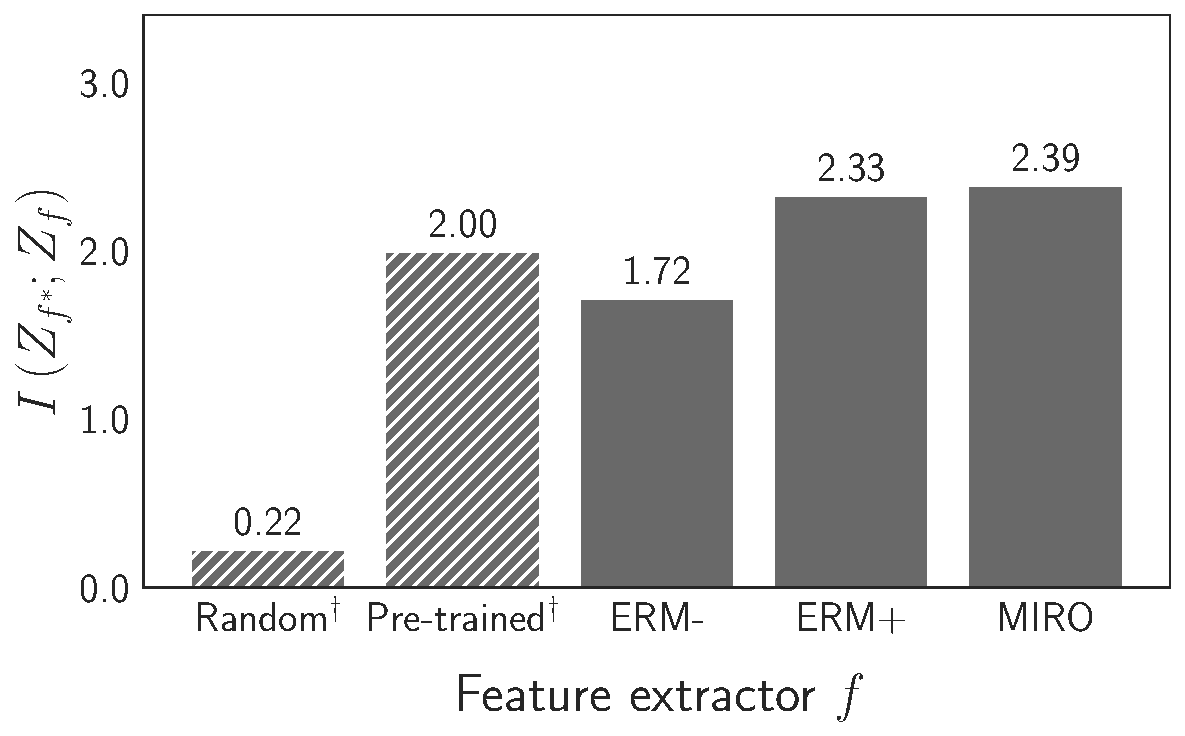
\includegraphics[width=\linewidth]{figures/mi/mi_resnet.pdf}
        \caption{\small ResNet-50}
        \label{fig:mi-resnet}
    \end{subfigure}%
    \hfill
    \begin{subfigure}{0.49\linewidth}
        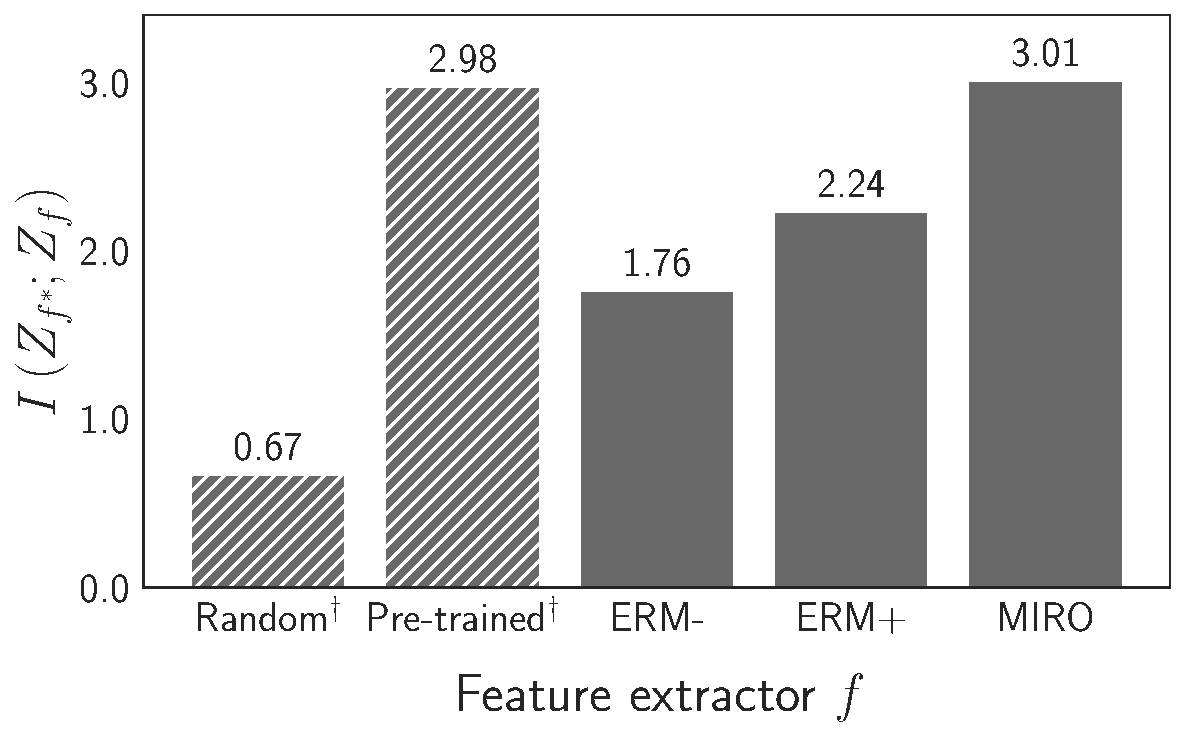
\includegraphics[width=\linewidth]{figures/mi/mi_swag.pdf}
        \caption{\small RegNetY-16GF}
        \label{fig:mi-regnet}
    \end{subfigure}%
    % \begin{subfigure}{0.53\linewidth}
    %     \includegraphics[width=\linewidth]{figures/mi/mi_all.pdf}
    %     \caption{\small All}
    %     \label{fig:mi-all}
    % \end{subfigure}
    \caption{\small \textbf{Mutual information $I\left( Z_{f^{*}}; Z_f \right)$ with oracle model.} The mutual information is estimated by MINE~\cite{belghazi2018mine} in \data{PACS}. Oracle model is trained using all of the four domains. \textit{Random} and \textit{Pre-trained} indicate random and pre-trained model initialization, respectively. \textit{ERM-} and \textit{ERM+} are trained from random and pre-trained model initialization, respectively. $\dagger$ indicates models without fine-tuning. The experiments are repeated with two pre-trained models: ImageNet 1.3M pre-trained ResNet-50 and Instagram 3.6B pre-trained RegNetY-16GF.}
    \label{fig:mi}
    % \vspace{-1em}
\end{figure}



% \begin{figure}
%     \centering
%     \includegraphics[width=0.7\columnwidth]{figures/mi_all.pdf}
%     \caption{\textbf{Mutual information with oracle model.} \textit{Random} is randomly initialized model, \textit{Scratch} is trained by ERM from \textit{Random}, and \textit{Pretrained} is initialized by pretrained model without training. \textit{ERM} and \textit{SIL} is initialized by pretrained model and trained by each method. $\dagger$ indicates RegNetY-16GF pretrained by SWAG is used and ResNet-50 pretrained in ImageNet is used for the others.}
%     \label{fig:mi}
% \end{figure}




\subsection{Mutual information analysis with the oracle model}
\label{subsection:mi_with_oracle}

Here, we empirically show how our approximation by pre-trained models is close to the oracle model and how our algorithm is effective to learn representations having high mutual information (MI) to the underlying oracle model. More specifically, we compare MI between the candidate models and the oracle model on the \pacs{} dataset.
% For the candidates, we choose ``Random'' networks (\ie, randomly initialized weights without any training), ``Pre-trained'' networks from ImageNet 1.3M and Instagram 3.6B (\ie, pre-trained ResNet-50 and RegNetY-16GF, respectively), fine-tuned models from ``Random'' network and ``Pre-trained'' networks (we name each model as ``ERM$-$'' and ``ERM$+$'', respectively), and models trained by our algorithm (\method).
Since the \emph{true} oracle model 
%(\ie, a model invariant to \emph{any} domain) 
is not achievable in practice, we train an oracle model by directly optimizing a model on the entire domains. We train two oracle models with ResNet-50 and RegNetY-16GF backbones, where the average validation accuracies across all domains
%of ResNet-50 and RegNetY-16GF oracle models 
are $97.2\%$ and $98.4\%$, respectively. We estimate MI between models by mutual information neural estimation (MINE) \cite{belghazi2018mine}. We describe the full details in Appendix \ref{subsec:mine}.

Figure \ref{fig:mi} illustrates the empirical MI between the candidate models and the oracle model.
In the figures, we first observe that the larger and more powerful pre-trained backbone (``Pre-trained'' in Figure \ref{fig:mi-regnet}) shows higher MI than the smaller backbone (``Pre-trained'' in Figure \ref{fig:mi-resnet}). Both pre-trained models consistently outperform ``Random'' in MI regardless of the backbone models. Our observations imply that a larger and stronger model is closer to the oracle model in terms of MI.
% We also observe that pre-trained models consistently show high mutual information with the oracle model compared to ``Random'' regardless of the backbone models.
Similarly, we observe that ERM$+$ always shows high MI than ERM$-$. However, interestingly, in Figure \ref{fig:mi-regnet}, we observe that fine-tuning significantly harms MI of the pre-trained model (``Pre-trained'' vs. ``ERM$+$'') when the pre-trained model becomes larger and more powerful. Our observation is aligned in the same line as the previous studies on fine-tuning of large models \cite{wortsman2021robust, kumar2022iclr_finetuning_distort}.
Lastly, in both scenarios of ImageNet pre-trained ResNet (Figure \ref{fig:mi-resnet}) and SWAG pre-trained RegNet (Figure \ref{fig:mi-regnet}), our \method{} shows the highest MI with the oracle model.
Note that MI with the oracle model may not be completely aligned with the DG performance, but in practice, we observed that the evaluation ranking of the candidates is the same as the MI ranking; \method{} scores the best, followed by ERM$+$ and ERM$-$. Detailed results are provided in Appendix \ref{subsec:relationship_mi_dg}.
% \jb{Note that higher MI does not guarantee higher DG performance, but we observed that the evaluation ranking of the candidates is the same as the MI ranking; \method{} scores the best, followed by ERM$+$ and ERM$-$. Detailed results are provided in Appendix.}


% Appendix?
\subsection{Features and encoders design}
% Here, we describe the design choices for the feature extractor $f$ for \method{}. We employ a multi-level structure to cope with the task shift between pre-training and fine-tuning, and simple encoder designs for the increased feature size.

\subsubsection{Multi-scale features.}
% One remaining question is which features to use. The naive solution is using the last high-level features, \ie, input features of the classifier. 
One can only use the last-level features for our regularization.
However, high-level features can include pre-training task-related information, often irrelevant to the target task. 
% Instead, we collect multi-scale features.
% Instead, we employ a multi-level structure, by collecting multi-scale features.
% Too much detail?
% Specifically, 
Instead,
we use the intermediate outputs by each model block, \ie, stem output, blocks 1, 2, 3, and 4 for ResNet \cite{he2016_cvpr_resnet} and RegNet \cite{radosavovic2020regnet}, and stem output, blocks 3, 6, 9, and 12 for ViT-B.
% the outputs from each quarter of the network body and the stem block as features. That is, the outputs of stem, block1, block2, block3, and block4 are collected for ResNet~\cite{he2016_cvpr_resnet}, and the outputs of stem, block3, block6, block9, and block12 are used for ViT-B~\cite{dosovitskiy2021vit} (ViT-B has 12 blocks in total).


\subsubsection{Design of the mean and variance encoders.} The multi-level structure increases the feature size, resulting in a computational cost increase. 
We alleviate the issue by employing 
% In order to alleviate this issue, we employ 
simple yet effective architectures, identity function for the mean encoder and a bias-only model with diagonal covariance for the variance encoder.
%whose diagonal term is $\sigma(Z_{f})$ and off-diagonal term is zero.
%to minimize additional computational cost from the multi-scale design. 
%The softplus function is adopted to restrict the output of the variance model to the positive number. 
We also tested more complicated architectures, but only computational cost was increased without performance improvement.